\documentclass[a4paper]{report}



    \usepackage[colorinlistoftodos]{todonotes}
 
	\usepackage[utf8]{inputenc}
	\usepackage[T1]{fontenc}
    \usepackage[frenchb]{babel}
    \usepackage{textcomp} 
	\usepackage[top=3cm,left=3cm,right=3cm,bottom=2cm]{geometry}
    \usepackage{lmodern}
    \usepackage{sectsty}
    \usepackage{nicefrac}
	\usepackage{graphicx}
    \usepackage{lastpage}
    \usepackage{fancyhdr}
    \usepackage{amsmath}
    \usepackage{amssymb}
    \usepackage{amsfonts}
    \usepackage{capt-of}
    \usepackage{caption}
    \usepackage{tikz}
    \usepackage{multirow}
	\usepackage{todonotes}    
    
    \usepackage{fancyvrb} % pour forcer les verbatim sur une seule page
    \usepackage{url}
    
    \usepackage{subfigure}
    %\usepackage{subcaption}
    
    \newcommand\matlab{MATLab\textsuperscript{\textregistered}}




\title{Premier jet du Rapport de projet de M1: Réseau periodiques et modes localisés }
%\subtitle{Basis of room acoustics: TP1}

\author{Thomas Lechat \& Alice Dinsenmeyer}

\begin{document}
\maketitle
\tableofcontents

\chapter*{Remerciements}

\chapter*{Abstract}

%intro : interet, problematique, contexte 
This study is about sound propagation in periodic structures, focusing on the case of a guide, periodically loaded by Helmholtz resonators, taking in account losses. The work on resonant acoustic meta-materials is closely linked to those in electromagnetism and in crystallography on lattice.\\~\\ %Historically, research on lattice has been more developed in this two field than in acoustics%historiquement, c'est ces deux derniers domaines dans lequel ça a été développé, donc moins en acoustique

This kind of structures is used for its ability to create a dispersive medium. Indeed, some frequencies passing through the lattice are absorbed for two reasons. One reason is that resonators absorb the energy at the frequencies near theirs resonances. Other frequency gaps, called Bragg gaps, are created by the periodicity that localise waves for witch the wave length is twice the distance between two resonators.\\~\\

Theoretical works and numerical simulations are leaded in this report in order to describe the frequency response for finite, infinite, disordered and ordered lattice. 

Then, using this dispersion and introducing a defect on one of the resonators, a phenomenon of localised wave is studied numerically and observed experimentally. For this purpose, the choice of the resonance frequency of the defect and its position in the lattice is carefully considered. If the defect resonate at a frequency cut by the lattice, the pressure wave generated cannot propagate and is restricted in the vicinity of the defect.\\~\\ 


%contribution aux recherche en non-lineaire.
Keywords: lossy periodic structures, dispersion, localised mode 


%methodologie : comment

%résultats principaux, conclusion, implication


\chapter*{Introduction}


La propagation dans les réseaux n'est pas un sujet nouveau: celui-ci a déjà été abordé en profondeur notamment dans des recherches en cristallographie et en électromagnétisme. Cependant sont pendant acoustique à fait l'objet de peut de recherches.

L'étude de la propagation acoustique dans les réseaux est un domaine complexe des lors que les éléments constitutif du réseau disposent de leurs propres fréquences de résonance. En effet, 2 types de bandes interdites sont alors présentes et peuvent interagir: les bandes de Bragg lié à la géométrie du réseau et les bandes interdites liés au comportement fréquentiel des éléments du réseau. Si on défaut est ajouté dans le réseau, il peut alors ce produire un phénomène de localisation de la pression dans le tube: c'est ce qu'on appelle un mode localisé (ou mode de défaut).

Ce travail s'inscrit dans le cadre de recherche sur les méta-matériaux composés de structures résonantes localisés. Ce genre de matériaux dispose de propriétés uniques tels que la réfraction négative ou encore des matériaux super-absorbant. Notre projet consiste à mieux comprendre le phénomène de mode localisé afin que des chercheurs puissent exploiter les résultats obtenues en y ajoutant des phénomènes d'acoustique non-linéaire.

\bigskip
Le but du projet est donc d'étudier la propagation dans un réseau composés de résonateurs de Helmholtz en prenant en compte les pertes visco-thermique intrinsèque à la propagation dans ce type de structure. Une fois la théorie sur les réseaux périodiques assimilé, une étude sur l'ajout d'un défaut dans le réseau sera effectuée. Des simulations seront confrontés à des mesures sur un réseau se trouvant au laboratoire d'acoustique de l'université du Maine.

%\begin{itemize}
%
%\item domaine de recherche: méta-matériaux, filtrage analogique, tout les phénomènes de propagation.
%\item Citation des sources => optique puis electromagnetique puis acoustique
%\item but: comprendre propagation dans réseau et visualisation expérimental de mode localisé
%\item plan: Approche théorique de la propa dans réseau ac, ajout de singularité pour mode localisé, expérimentation
%\end{itemize}
\chapter{Théorie d'un réseau acoustique fini constitué de résonateurs de Helmholtz}
Ce chapitre a pour but de caractériser le champ de pression dans un guide sur lequel des résonateurs de Helmholtz sont placés en dérivation, espacés régulièrement d'une longueur $L$. On dispose pour cela d'un banc de mesure représenté en figure ~\ref{schema_infini}. Une simulation de la propagation dans le réseau pourra donc être confronté à une expérience.

\begin{figure}[!ht] \centering
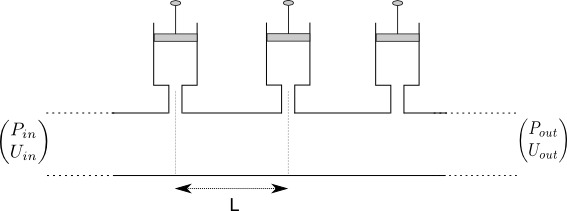
\includegraphics[scale=0.5]{./images_chp1/schema_reseau_infini.png}
\caption{\label{schema_infini} Schéma du réseau de résonateurs de Helmholtz.}
\end{figure}

\paragraph{Notations}
Le guide principal a pour section $S$ ; le col des résonateurs a pour longueur $L_{n}$ et pour section $S_{n}$ ; la cavité des résonateurs a pour longueur $L_{c}$ et pour section $S_{c}$. Par la suite, on note $\rho$ la masse volumique de l'air et $c$ la célérité du son dans l'air.

\section{Mise sous forme matricielle}
On s’intéresse ici a la mise sous forme matricielle du problème de la propagation acoustique dans le réseau periodique vu ci-dessus. Le but est de mettre en relation les pressions et débits en entrée du système ($P_{in}$ et $U_{in}$) avec ceux en sortie ($P_{out}$ et $U_{out}$) sous la forme suivante:
\begin{equation}
\begin{pmatrix} P_{out} \\ U_{out} \end{pmatrix} =\begin{pmatrix} a & b \\ c & d \end{pmatrix}^N \begin{pmatrix} P_{in} \\ U_{in} \end{pmatrix} = \begin{pmatrix} A & B \\ C & D \end{pmatrix} \begin{pmatrix} P_{in} \\ U_{in} \end{pmatrix} .
\end{equation}

Cette matrice dispose en effet de propriétés intéressantes et l'étude du système sera grandement facilité par ce formalise. De plus, les simulations sont faciles à mettre en œuvre dès lors que celle ci est connue.

Pour cela, les 2 éléments du réseau (guide et résonateur) doivent être mis sous forme matricielle puis multipliés.

\subsection{Le guide d'onde}
La solution de la propagation dans un guide d'onde peux être facilement déduite de l'équation d'onde suivante :
\begin{equation}
\frac{\partial ^2 p}{\partial x^2} -\frac{1}{c^{2}} \frac{\partial ^2 p}{\partial t^2}= 0
\end{equation}\todo[inline]{Dire qu'on est en 1D (d'où dx) car guide long et BF}

On se place en régime harmonique et on note $\Gamma = jk$ la constante de propagation du système. D’où les solutions (vitesses calculées avec l'équation d'Euler:

\begin{eqnarray*}
\begin{cases}
p(x_1)  =  C_1 e^{-\Gamma x_1} + C_2 e^{\Gamma x_1} \\
v(x_1)  =  -\frac{1}{j\omega\rho} [ -\Gamma C_1 e^{-\Gamma x_1} + \Gamma e^{\Gamma x_1}]\\
p(x_2)  =  C_1 e^{-\Gamma x_2} + C_2 e^{\Gamma x_2} \\
v(x_2)  =  -\frac{1}{j\omega\rho} [ -\Gamma C_1 e^{-\Gamma x_2} + \Gamma e^{\Gamma x_2}]
\end{cases}
\end{eqnarray*}
 
On pose $x_1 - x_2 = L$. Tous calculs faits, on trouve finalement:
\begin{eqnarray*}
\begin{pmatrix} p(x_1) \\ v(x_1) \end{pmatrix} = \begin{pmatrix} \cosh(kL) & \frac{j\omega\rho}{k} \sinh(k L) \\  \frac{k}{j\omega\rho}\sinh(k L) & \cosh(k L) \end{pmatrix} \begin{pmatrix} p(x_2) \\ v(x_2) \end{pmatrix}
\end{eqnarray*}

La première fréquence de coupure du guide est donc d'environ $4kHz$ pour les dimensions du réseau que nous considérons. Dans la suite, on supposera donc que seul le mode plan est propagatif. Les simulations et mesures ne seront donc faite que sur une bande de fréquences allant de $0$ à $1~kHz$.

\subsubsection{Ajout des pertes}
\todo[inline]{source biblio à citer}

Pour prendre en compte les pertes, on modifie l'expression de la constante de propagation et de l'impédance caractéristique. Les expressions sont donc:
\begin{eqnarray*}
 k =  \frac{\omega}{c_0} \left( 1 + \frac{\beta}{s}(1+(\gamma-1)/ \chi \right) \\
 Z_c =  \frac{\rho c_0}{S} \left( 1 + \frac{\beta}{s}(1-(\gamma-1)/ \chi \right) 
\end{eqnarray*}

Dans ces expressions, on a:
\begin{itemize}
 \item  $s=R/ \delta$ avec $\delta = \sqrt{\frac{2 \mu}{\rho \omega}}$
 \item  $\chi = \sqrt{P_r}$ ou $P_r$ est le nombre de Prandtl
 \item $\beta = (1-j)/\sqrt{2}$ 
 \item $\mu$ la viscosité de l'air
\end{itemize}

Du fait de la géométrie assez complexe du système, ces pertes ne peuvent pas être négligées comme cela peux être souvent le cas en acoustique.

\subsection{Impédance d'entrée d'un résonateur}
Le résonateur de Helmholtz est considéré dans le réseau comme un changement ponctuel d'impédance. Cette impédance, notée $Z_{r}$ peut être calculée en utilisant le même formalisme matriciel que précédemment.



 %Cette impédance peux être calculée via la formule de l'impédance ramenée ~\ref{imp_ramenee}. De plus, les dimensions utilisées dans la suite sont corrigées afin de prendre en compte les corrections de longueurs liés à la géométrie du problèmes. Ces formules de corrections sont disponibles en annexe 2.
%\begin{eqnarray}
%Z{x_1}=\frac{jZ_c tan(kL)+Z_{x_2}}{1+j\frac{Z_{x_2}}{Z_c}tan(kL)}.
%\label{imp_ramenee}
%\end{eqnarray}

On suppose que le résonateur est constitué de 2 guides à parois rigides d'impédance caractéristique $Z_{n}=\rho c/S_{n}$ pour le col et $Z_{c}=\rho c /S_{c}$ pour la cavité. La matrice de transfert mettant en relation les pression et débit à l'entrée du résonateur $P_e$ et $U_e$ et les pression et débit au niveau de la paroi extrême $P_s$ et $U_s=0$ est de la forme :
\begin{eqnarray*}
\begin{pmatrix} P_e \\U_e \end{pmatrix} & = & \begin{pmatrix} \cos(k L_n) & j Z_{n} \sin(k L_n) \\ \frac{1}{Z_{n}} \sin(k L_n) & \cos(k L_n) \end{pmatrix} \begin{pmatrix} \cos(k L_c) & j Z_{c} \sin(k L_c) \\ \frac{1}{Z_{c}} \sin(k L_c) & \cos(k L_c) \end{pmatrix} \begin{pmatrix} P_s \\ 0  \end{pmatrix} \\
\begin{pmatrix} P_e \\U_e \end{pmatrix} & = & \begin{pmatrix} r_1 & r_2 \\ r_3 & r_4 \end{pmatrix} \begin{pmatrix} P_1 \\ 0  \end{pmatrix} \\
~ & \Leftrightarrow & Z_{r}	 = \frac{P_e}{U_e}= \frac{r_1}{r_3}
\end{eqnarray*}

\paragraph{Correction de longueur}
La longueur effective du col est sujet à une correction présentée en annexe \todo[inline]{correction liée à quoi, détaille-t-on ce passage ?}

En ajoutant un résonateur en parallèle au guide, il y a toujours continuité des pressions mais plus des vitesses. La matrice de transfert pression-débit pour un résonateur dans le réseau est alors la suivante :

\begin{eqnarray*}
M_{r} = \begin{pmatrix} 1 &  0 \\ 1 /Z_{r} & 1  \end{pmatrix}\\
\end{eqnarray*}

\section{Étude du réseau fini}

Une fois les matrices de guide et de résonateur connues, il suffit alors de les multiplier afin d'obtenir la matrice d'une cellule du réseau. C'est sur l'étude de cette matrice que se basent les analyses de cette section. 

Dans la suite les paramètres de la simulation sont ceux de l'expérience dont nous disposons. Ces paramètres sont disponible en annexe 2.

\subsection{Équation de dispersion}
La matrice de transfert l'équation de dispersion pour le réseau à N cellules s'écrit alors : 
\begin{equation}
\cos(NkL) = \frac{A+D}{2} 
\end{equation}

Ainsi, on peut remonter à une expression de $kL$ en fonction de la fréquence. En particulier, les zones où $kL$ devient imaginaire nous intéressent particulièrement car cela induit une décroissance exponentielle de l'onde de propageant dans le guilde (onde évanescente). Ces bandes sont visibles sur la figure~\ref{bande_bragg} et sont appelées les bandes de Bragg.

\todo{une figure de l’équation de dispersion avec bande de bragg}

\subsection{Réflexion et transmission du réseau}
Le coefficient de réflexion et de transmission du réseau complet peut être calculé de la manière suivante [\todo[inline]{Source biblio}] : 
\begin{eqnarray}
T & = & \frac{2}{A + B/Z_c + C Z_c + D} \\
R & = & \frac{A + B / Zc_ - C Z_c -D}{A + B/Z_c + C Z_c + D} 
\end{eqnarray}

On trace ces coefficients en fonction de la fréquence (figure~\ref{ex_coef_RT}) ainsi que l'admittance des résonateurs utilisés. Il apparaît que la transmission chute pour trois bandes de fréquence : à la résonance du résonateur de Helmholtz, à celle de sa cavité et à la première bande de Bragg.

\subsection{Bande de Bragg}
Ces bandes sont visibles dès que des singularités apparaissent de manière periodique. L'énergie de l'onde est reste contenue entre chaque élément du fait que la longueur d'onde correspond à la moitié de l'espacement entre 2 éléments. 

Pour un espacement entre éléments de longueur $L=0.1~m$, la bande de Bragg se situe autour de la fréquence $f_{b} = \frac{c}{2L} = 1715 Hz$. On constate sur la figure~\ref{ex_coef_RT} que ces bandes de Bragg sont bien présentes à la fréquence indiquée ainsi qu'a ses multiples (chute de la transmission et réflexion maximale).
 

\subsection{Bande interdites liés aux résonateurs}
L'équation de dispersion est cependant plus difficile à analyser qu'il n'y parait en raison des résonateurs qui constituent réseau. Ceux-ci ont une impédance négligeable dès lors que la fréquence d'analyse se trouve suffisamment éloigné des fréquences de résonances. 

De plus le résonateur étant par nature un système résonant, il peut lui aussi induire une absorption de l'énergie de l'onde sur certaines fréquences. Sur la figure~\ref{ex_coef_RT}, ces bandes interdites sont aussi présentes: elles se trouvent là ou l'admittance du résonateur est maximale. A ces fréquences, on a bien une chute de la transmission.

\begin{figure}
\centering
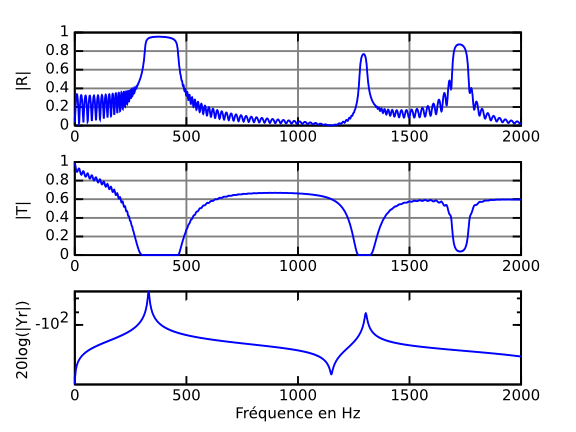
\includegraphics[scale=0.7]{./images_chp1/ex_coef_rapport.png}
\caption{\label{ex_coef_RT} Coefficient de réflexion (en haut) et de transmission (au milieu) pour un réseau de 60 résonateurs avec $L_c=14~cm$. En bas : Impédance d'entrée du résonateur.}
\end{figure}

\subsection{Cas désordonné}

\subsubsection{Désordre sur le volume des cavités}

Afin d'étudier succinctement l'effet d'un désordre sur le volume des cavités du résonateur, une simulation numérique est réalisée pour des longueurs de cavité suivant une loi normale. Comme précédemment, les résonateurs sont arbitrairement au nombre de 60 et sont séparés d'une distance $L=0.1$ m. La figure~\ref{chaos10} présente les coefficients de transmission et de réflexion pour une longueur de cavité moyenne de $\bar{L_c}=14$ cm et un écart-type  de $\sigma = 1$ cm.


Dans le cas d'un écart-type élevé, le désordre a pour principal effet d'élargir la bande interdite liée à la seconde résonance des résonateurs (résonance de la cavité). La bande de Bragg n'est pas impactée puisque le désordre touche le volume des cavités et non l'espacement des résonateurs.

\paragraph{Désordre lié aux conditions expérimentales}
Dans l'expérience menée plus loin, le volume des résonateur est fixé manuellement. La question de l'impact de l'erreur commise par la mise en place de l'expérience est donc directement liée à l'étude de désordre dans le réseau. On estime que la longueur des cavités va suivre une loi normale d'écart-type 2 mm et de longueur moyenne $\bar{L_c}=14$ cm. La figure~\ref{chaos2} montre alors que ce désordre n'a qu'une faible influence sur le coefficient de réflexion. 


\begin{figure}[!h]
	\begin{minipage}{0.45 \textwidth}
		\centering
		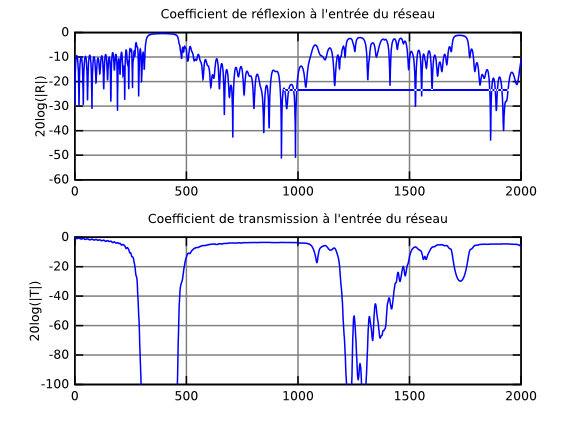
\includegraphics[scale=0.5]{./images_chp1/chaos_10mm.png}
		\caption{\label{chaos10} Coefficient de réflexion (en haut) et de transmission (en bas) pour un réseau de 60 résonateurs avec $\bar{L_c}=14$~cm et $\sigma =1$ cm.}
	\end{minipage}
\hspace{0.5cm}
	\begin{minipage}{0.45 \textwidth}
		\centering
		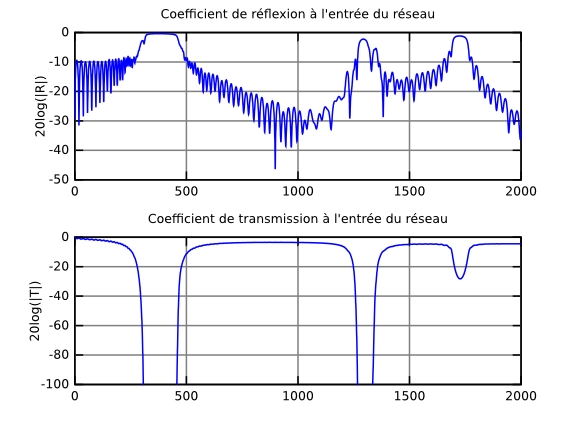
\includegraphics[scale=0.5]{./images_chp1/chaos_2mm.png}
		\caption{\label{chaos2} Coefficient de réflexion (en haut) et de transmission (en bas) pour un réseau de 60 résonateurs avec $\bar{L_c}=14$~cm et $\sigma=2$ mm.}
	\end{minipage}
\end{figure}



\subsubsection{Désordre sur la position des résonateurs}
La même étude est menée sur le désordre lié à la conception du banc de mesure et aux défauts de position des résonateur. La configuration du réseau est la même.
Les figures~\ref{chaospos10} et~\ref{chaospos2} montrent l'effet d'un désordre plus ou moins grand sur la réflexion et la transmission.

\begin{figure}[h!]
	\subfigure[\label{chaospos10}$\sigma=1$ cm]{
		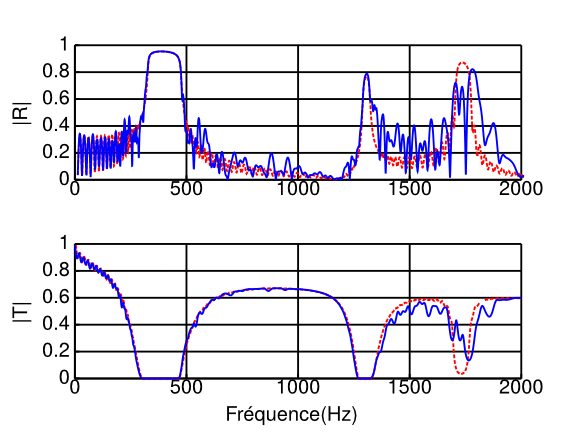
\includegraphics[scale=0.5]{./images_chp1/chaos_position_grand.png}
	}
	\subfigure[\label{chaospos2}$\sigma=2$ mm]{
		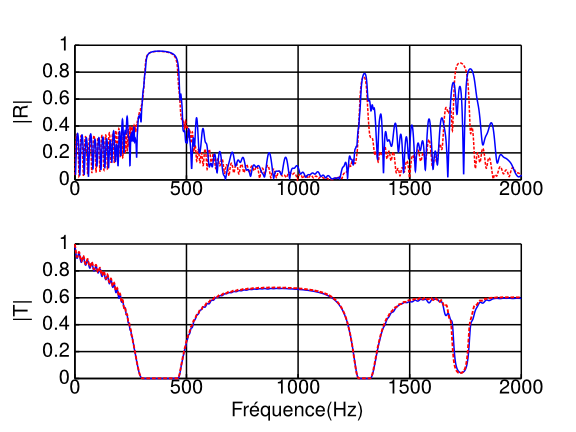
\includegraphics[scale=0.5]{./images_chp1/chaos_position_petit.png}
	}
	\caption{Coefficients de réflexion (en haut) et de transmission (en bas) pour un réseau de 60 résonateurs avec $\bar{L}=14$ cm.}
\end{figure}

Le désordre a pour principal effet d'augmenter la transmission au niveau de la bande de Bragg. Pour un désordre grand, l'effet du réseau n'est plus visible, puisque la bande interdite de Bragg va jusqu'à disparaître.

Le désordre d'écart-type 2 mm est supérieur à celui estimé pour la réalisation du banc de mesure et est cependant moindre. On considère donc qu'il est négligeable par la suite.




\chapter{Ajout d'une singularité dans le réseau}
La seconde partie de ce projet est une étude portant sur l'observation d'un mode localisé dans le réseau précédemment étudié. Pour cela, un résonateur est modifié de façon à créer une singularité dans le réseau. \\


Le banc de manipulation utilisé est le même que celui de la thèse~\cite{these_richoux} qui a servi de support au projet. Il ne permet de modifier que la longueur des cavités des résonateurs et non leur position. C'est donc en changeant ce paramètre que sera introduite et étudiée la singularité. La longueur de la cavité singulière est notée $L_{c_{s}}$.\\

En fonction du choix de la longueur de la cavité singulière, et donc de la fréquence de résonance du résonateur associé, différents phénomènes peuvent être observés. 

\section{Étude de l'influence de la fréquence de résonance du défaut}
Le réseau étudié a un comportement complexe d'un point de vue fréquentiel. Il est donc important de différencier les cas suivant la fréquence de résonance du défaut. Deux cas de figure sont représentés sur le schéma \ref{schema_singu1} : celui pour lequel la résonance du défaut est dans une bande interdite et celui où elle est dans une bande passante.

\begin{figure}[!h]
\centering
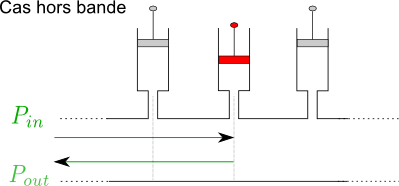
\includegraphics[scale=0.5]{images_chp2/schema_singu1.png} \hfill
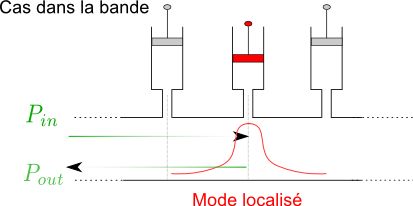
\includegraphics[scale=0.5]{images_chp2/schema_singu2.png}
\caption{\label{schema_singu1} Schémas de la configuration avec une singularité dans une bande interdite  et hors bande interdite.}
\end{figure}




\subsection{Cas du défaut hors bandes interdites}

Le cas le plus simple d'une singularité dans le réseau est celui où cette singularité se trouve hors de la bande de Bragg ou des bandes liées aux autres résonateurs (la fréquence de résonance de la singularité est dans une bande passante). La singularité crée un changement d'impédance brutal dans le réseau à sa fréquence de résonance car alors l'impédance du résonateur est maximale. Dans ce cas, la pression dans le réseau après la singularité est nulle : l'onde est totalement réfléchie. Ce résultat est visible sur la figure~\ref{defaut_hb}. Cette figure est une simulation de l'amplitude de la pression dans le réseau, excité par un sinus à la fréquence de résonance du défaut.	Les lignes noires indiquent l'emplacement des résonateurs (de longueur de cavité 16 cm) et la ligne rouge indique l'emplacement du défaut de longueur de cavité 7.1 cm.

La pression est calculée en chaque point du réseau par rétro-propagation en partant d'une terminaison anéchoïque à la fin du réseau. Les amplitudes visibles au niveau de la source n'ont donc pas nécessairement de réalité physique. On s'intéresse surtout à l'enveloppe du signal plus qu'aux ordres de grandeurs.


\begin{figure}[!h]
\centering
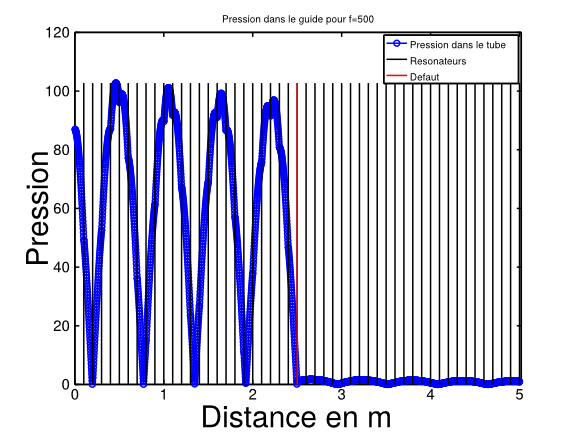
\includegraphics[scale=0.5]{images_chp2/horsbande_50RH_500Hz_71mm.png}
\caption{\label{defaut_hb} Visualisation de la pression dans le réseau avec un défaut dont la fréquence se trouve dans une bande passante. La fréquence d'excitation est celle du défaut (500 Hz). Celui-ci se trouve en 25\textsuperscript{ème} position dans un réseau de 50 résonateurs espacés de 10 cm.}
\end{figure}

\bigskip
On constate bien une chute de la pression au niveau de la singularité. Excité à sa fréquence de résonance, le résonateur défectueux entraîne une forte absorption. Ici, les pertes sont prises en compte : une fraction de l'onde incidente se propage donc dans le réseau après le défaut.



\subsection{Cas du défaut dans une bande interdite}

Si la fréquence de résonance du défaut se trouve dans une bande interdite, on a alors une localisation de l'onde au niveau du défaut. En effet, la propagation n'est pas possible de part et d'autre du défaut dans le réseau (ondes évanescentes). La fraction de l'onde incidente qui s'est propagée jusqu'au défaut excite ce dernier mais reste piégée du fait que ce défaut se trouve au milieu du réseau. On obtient alors un mode localisé : la pression est élevée à un endroit du guide et y reste confinée.
\bigskip


Du fait que cette pression soit localisée, elle n'a pas d'influence sur le coefficient de transmission sauf dans le cas d'un petit réseau où l'on peut supposer que l'étalement du mode localisé est suffisamment grand au regard de la taille du réseau pour atteindre les bords de celui-ci. Ce genre de phénomène est donc difficile à observer; cependant une simulation peut aider à en comprendre les concepts clés.
\bigskip

Comme précédemment, on trace sur la figure \ref{defaut_dansb} la pression dans le tube pour un défaut dont la résonance se trouve dans une bande interdite. Le réseau est excité à la fréquence du mode localisé. Cette fréquence résulte d'un couplage entre la singularité et le réseau. Elle peut être retrouvée expérimentalement car c'est la fréquence à laquelle la pression est maximale au niveau de la singularité. Elle peut aussi se retrouver sur le coefficient de réflexion : comme le montre la courbe de droite de la figure~\ref{defaut_dansb}, le coefficient de réflexion est très faible pour une fréquence donnée au milieu de la bande interdite. Cette fréquence correspond à celle du mode recherché.


\begin{figure}[!h]
\centering
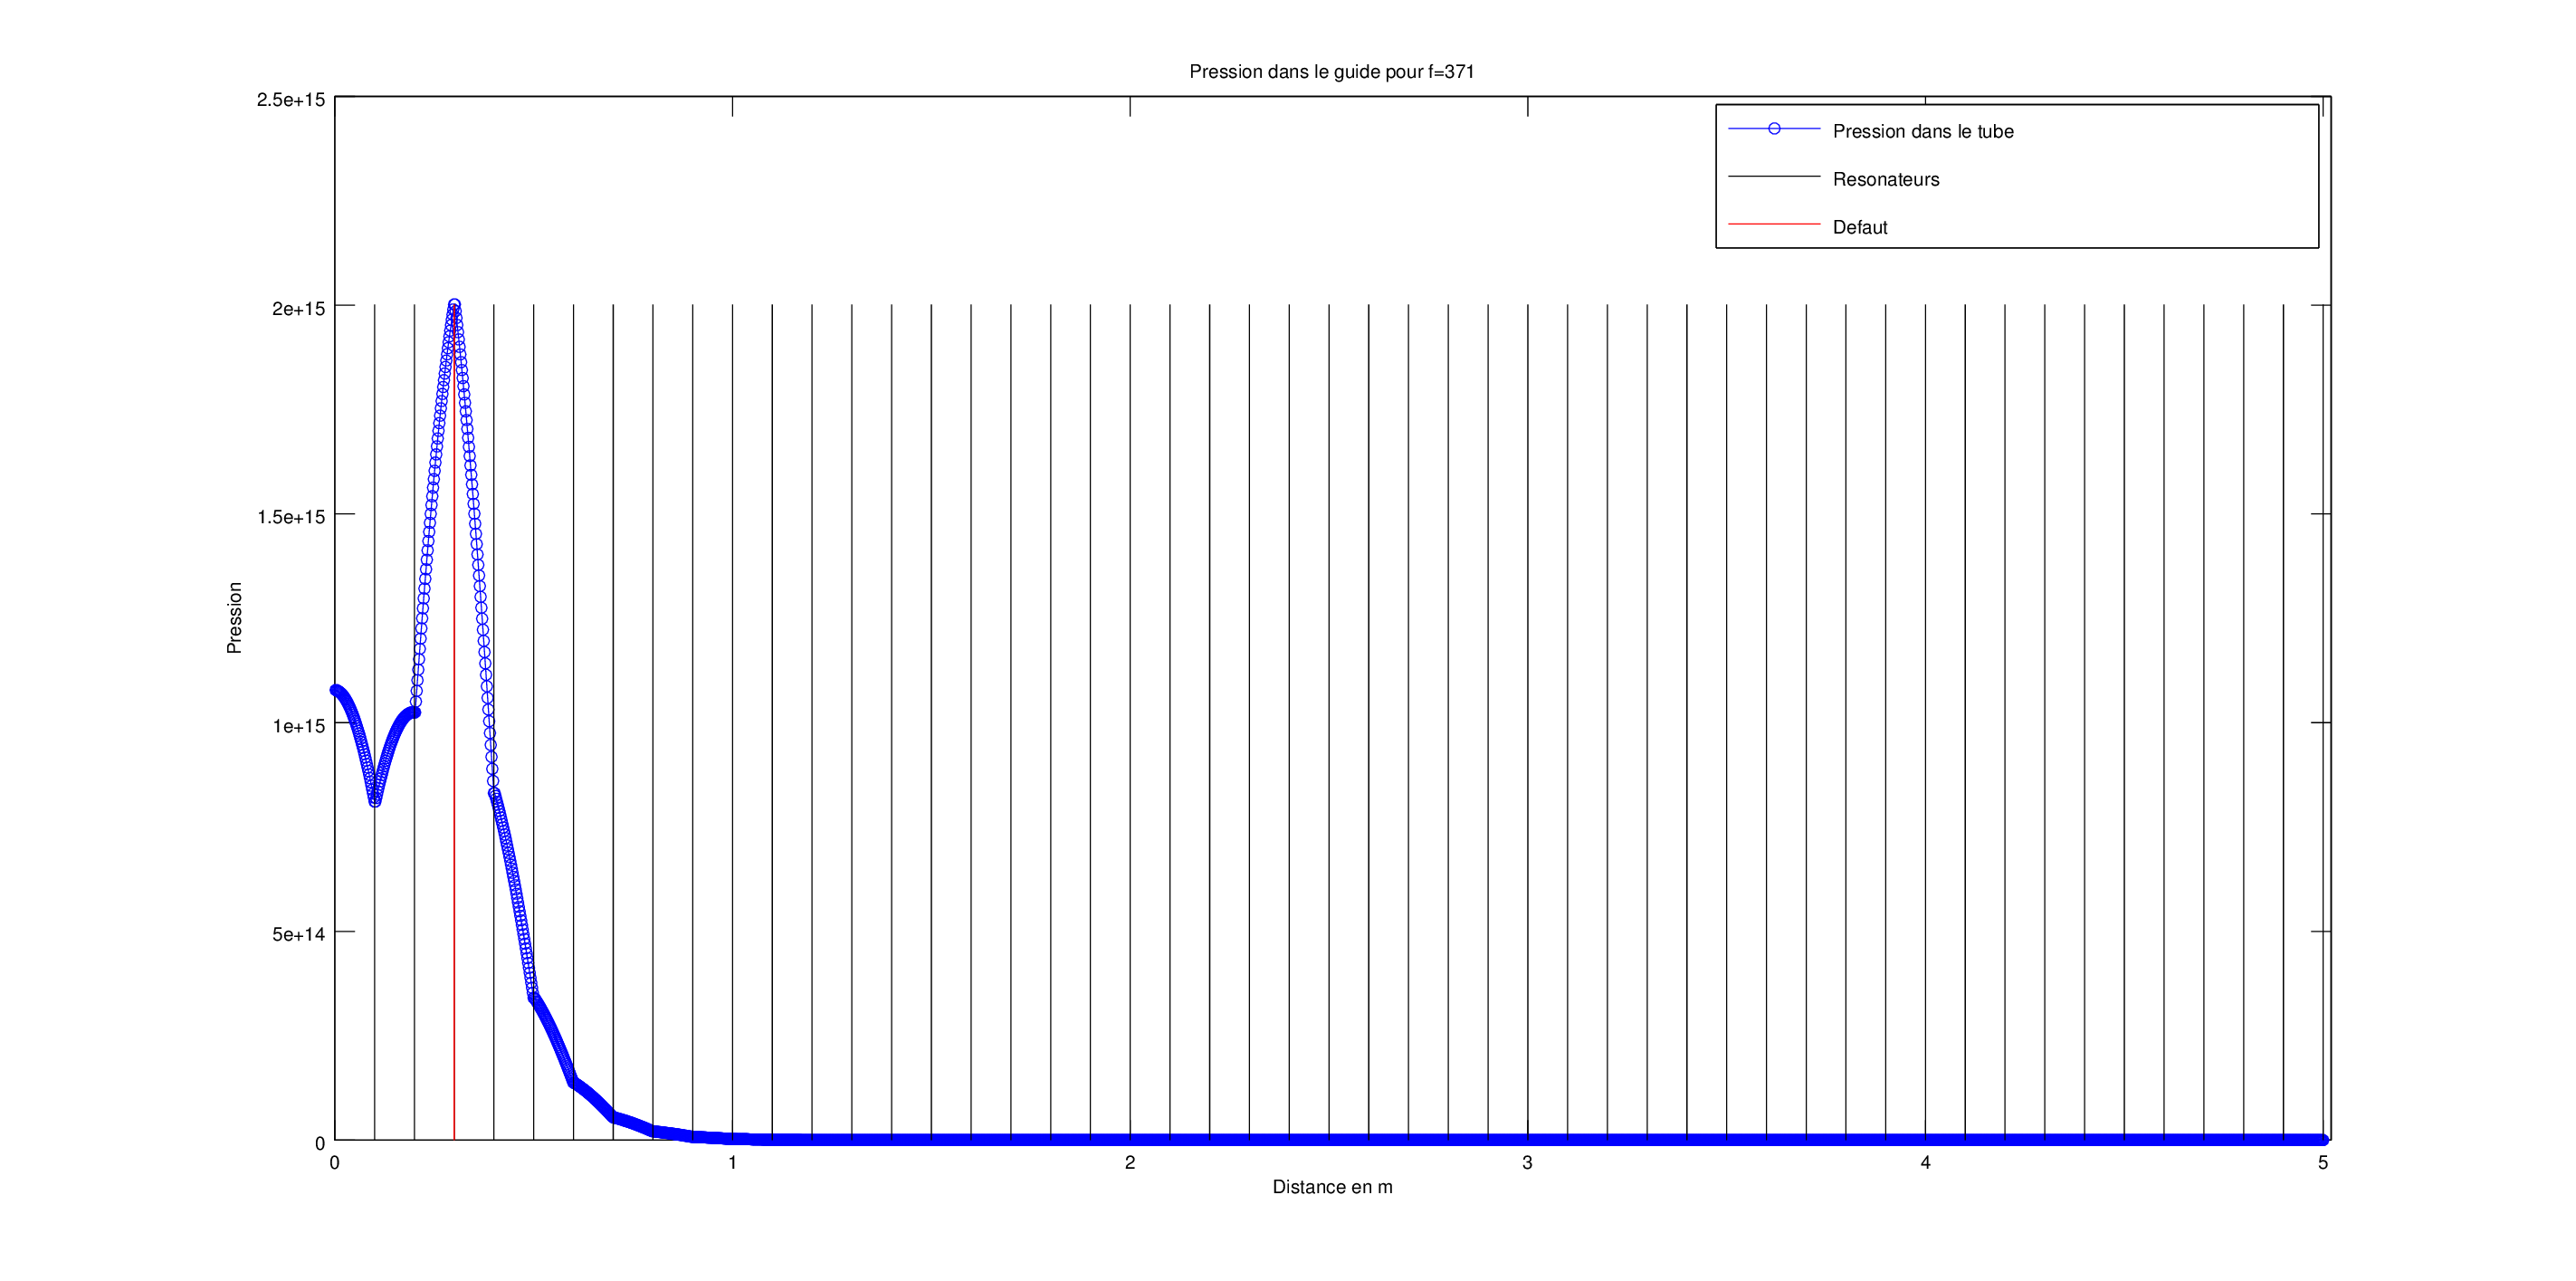
\includegraphics[height=6cm]{images_chp2/visu_pression_favo2.png}
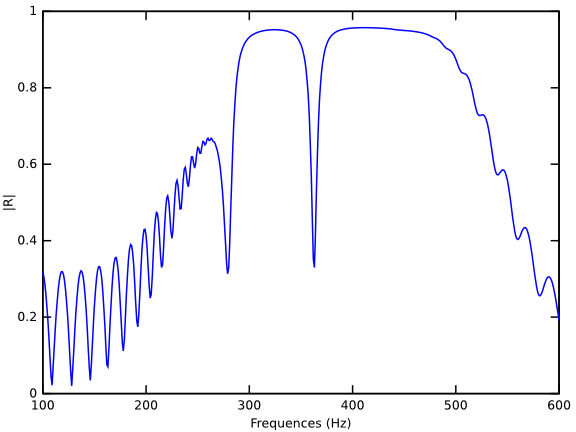
\includegraphics[height=5cm]{images_chp2/reflexion_50HR16_pos3_8cm.png}
\caption{\label{defaut_dansb} À gauche : Visualisation de la pression dans le réseau avec un défaut dont la fréquence se trouve dans une bande interdite ($L_{c_{s}}=8cm$. La fréquence d'excitation est à 371 Hz. Le défaut se trouve en 3\textsuperscript{ème} position dans un réseau de 50 résonateurs espacés de 10 cm.\\ À droite : Coefficient de réflexion pour le même réseau.}
\end{figure}


\section{Étude de l'influence de la position du défaut}
La position du défaut est elle aussi très importante afin de pouvoir générer un mode localisé: le défaut doit être suffisamment proche de la source afin d'être excité par les ondes évanescentes mais pas trop proche des bords car alors il n'est plus complètement localisé.

La figure~\ref{pos_singu} représente le coefficient de transmission pour un réseau constitué de 5 résonateurs en fonction de la position du défaut ($L_{c_{s}}=6.5 cm$). Il apparaît clairement que quand le défaut est en position 2 ou 3, une hausse de la transmission est visible autour de 390 Hz. Cette fréquence est celle du mode localisé. 

\begin{figure}[!h]
	\centering
	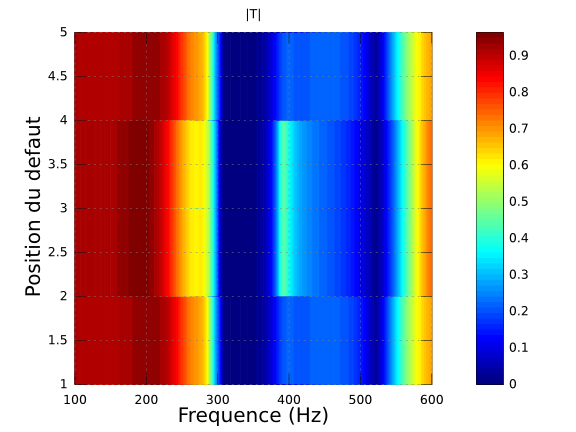
\includegraphics[scale=0.5]{images_chp2/pos_singu.png}
	\caption{Coefficient de transmission en fonction de la position du défaut et de la fréquence d'excitation.\label{pos_singu}}
\end{figure}

Dans la partie suivante, l'objectif est de visualiser expérimentalement ce mode localisé. Cette simulation numérique montre donc qu'il faut choisir judicieusement la position du résonateur défectueux ainsi que la fréquence d'excitation du réseau.
\chapter{Visualisation expérimentale d'un mode localisé}
Comme vu précédemment, un défaut dans le réseau provoque un mode localisé. L'objectif est ici de mettre en évidence ce phénomène de manière expérimentale.\\


Un mode localisé dans un tel réseau est à la fois difficile à générer et à observer, expérimentalement comme numériquement. La fréquence de résonance du défaut doit se trouver sur le bord intérieur d'une bande interdite afin de pouvoir la visualiser sur les coefficients de transmission et réflexion. En effet, la propagation de l'onde dans le réseau se fait sur une longueur réduite : la bande interdite rend la décroissance de l'onde exponentielle. Par conséquent, la fréquence de résonance du défaut et la position du défaut par rapport à la source sont cruciales. De plus, une fois le mode généré, il ne peut être observé que très localement et si le réseau est trop grand, il n'est alors pas visible sur les coefficients de transmission et de réflexion qui sont issus de mesures à l'entrée et la sortie du réseau.


\section{Protocole expérimental}
Le banc de mesure utilisé est constitué d'un tuyau perforé de 60 trous sur lesquels peuvent être fixés soit des résonateurs de longueurs de cavité variables (les dimensions sont présentes en annexe), soit des bouchons (cf figure~\ref{photo_manip}). La source utilisée est celle du capteur d'impédance (piézoélectrique). Celui-ci est préalablement calibré, puis fixé à une des extrémités du réseau et est reliée à une carte d'acquisition piloté par le logiciel spécialisé du CTTM\footnote{Centre de Transfert de Technologie du Mans}. Ce capteur dispose de 2 microphones et permet donc de calculer directement le coefficient de réflexion du réseau. Afin de pouvoir calculer le coefficient de transmission, un autre microphone (B\&K 2669, calibré) amplifié (GRAS 12AQ) est ajouté à l'autre extrémité du réseau, $10~cm$ après le dernier résonateur.


\begin{figure}[!h]
	\centering
	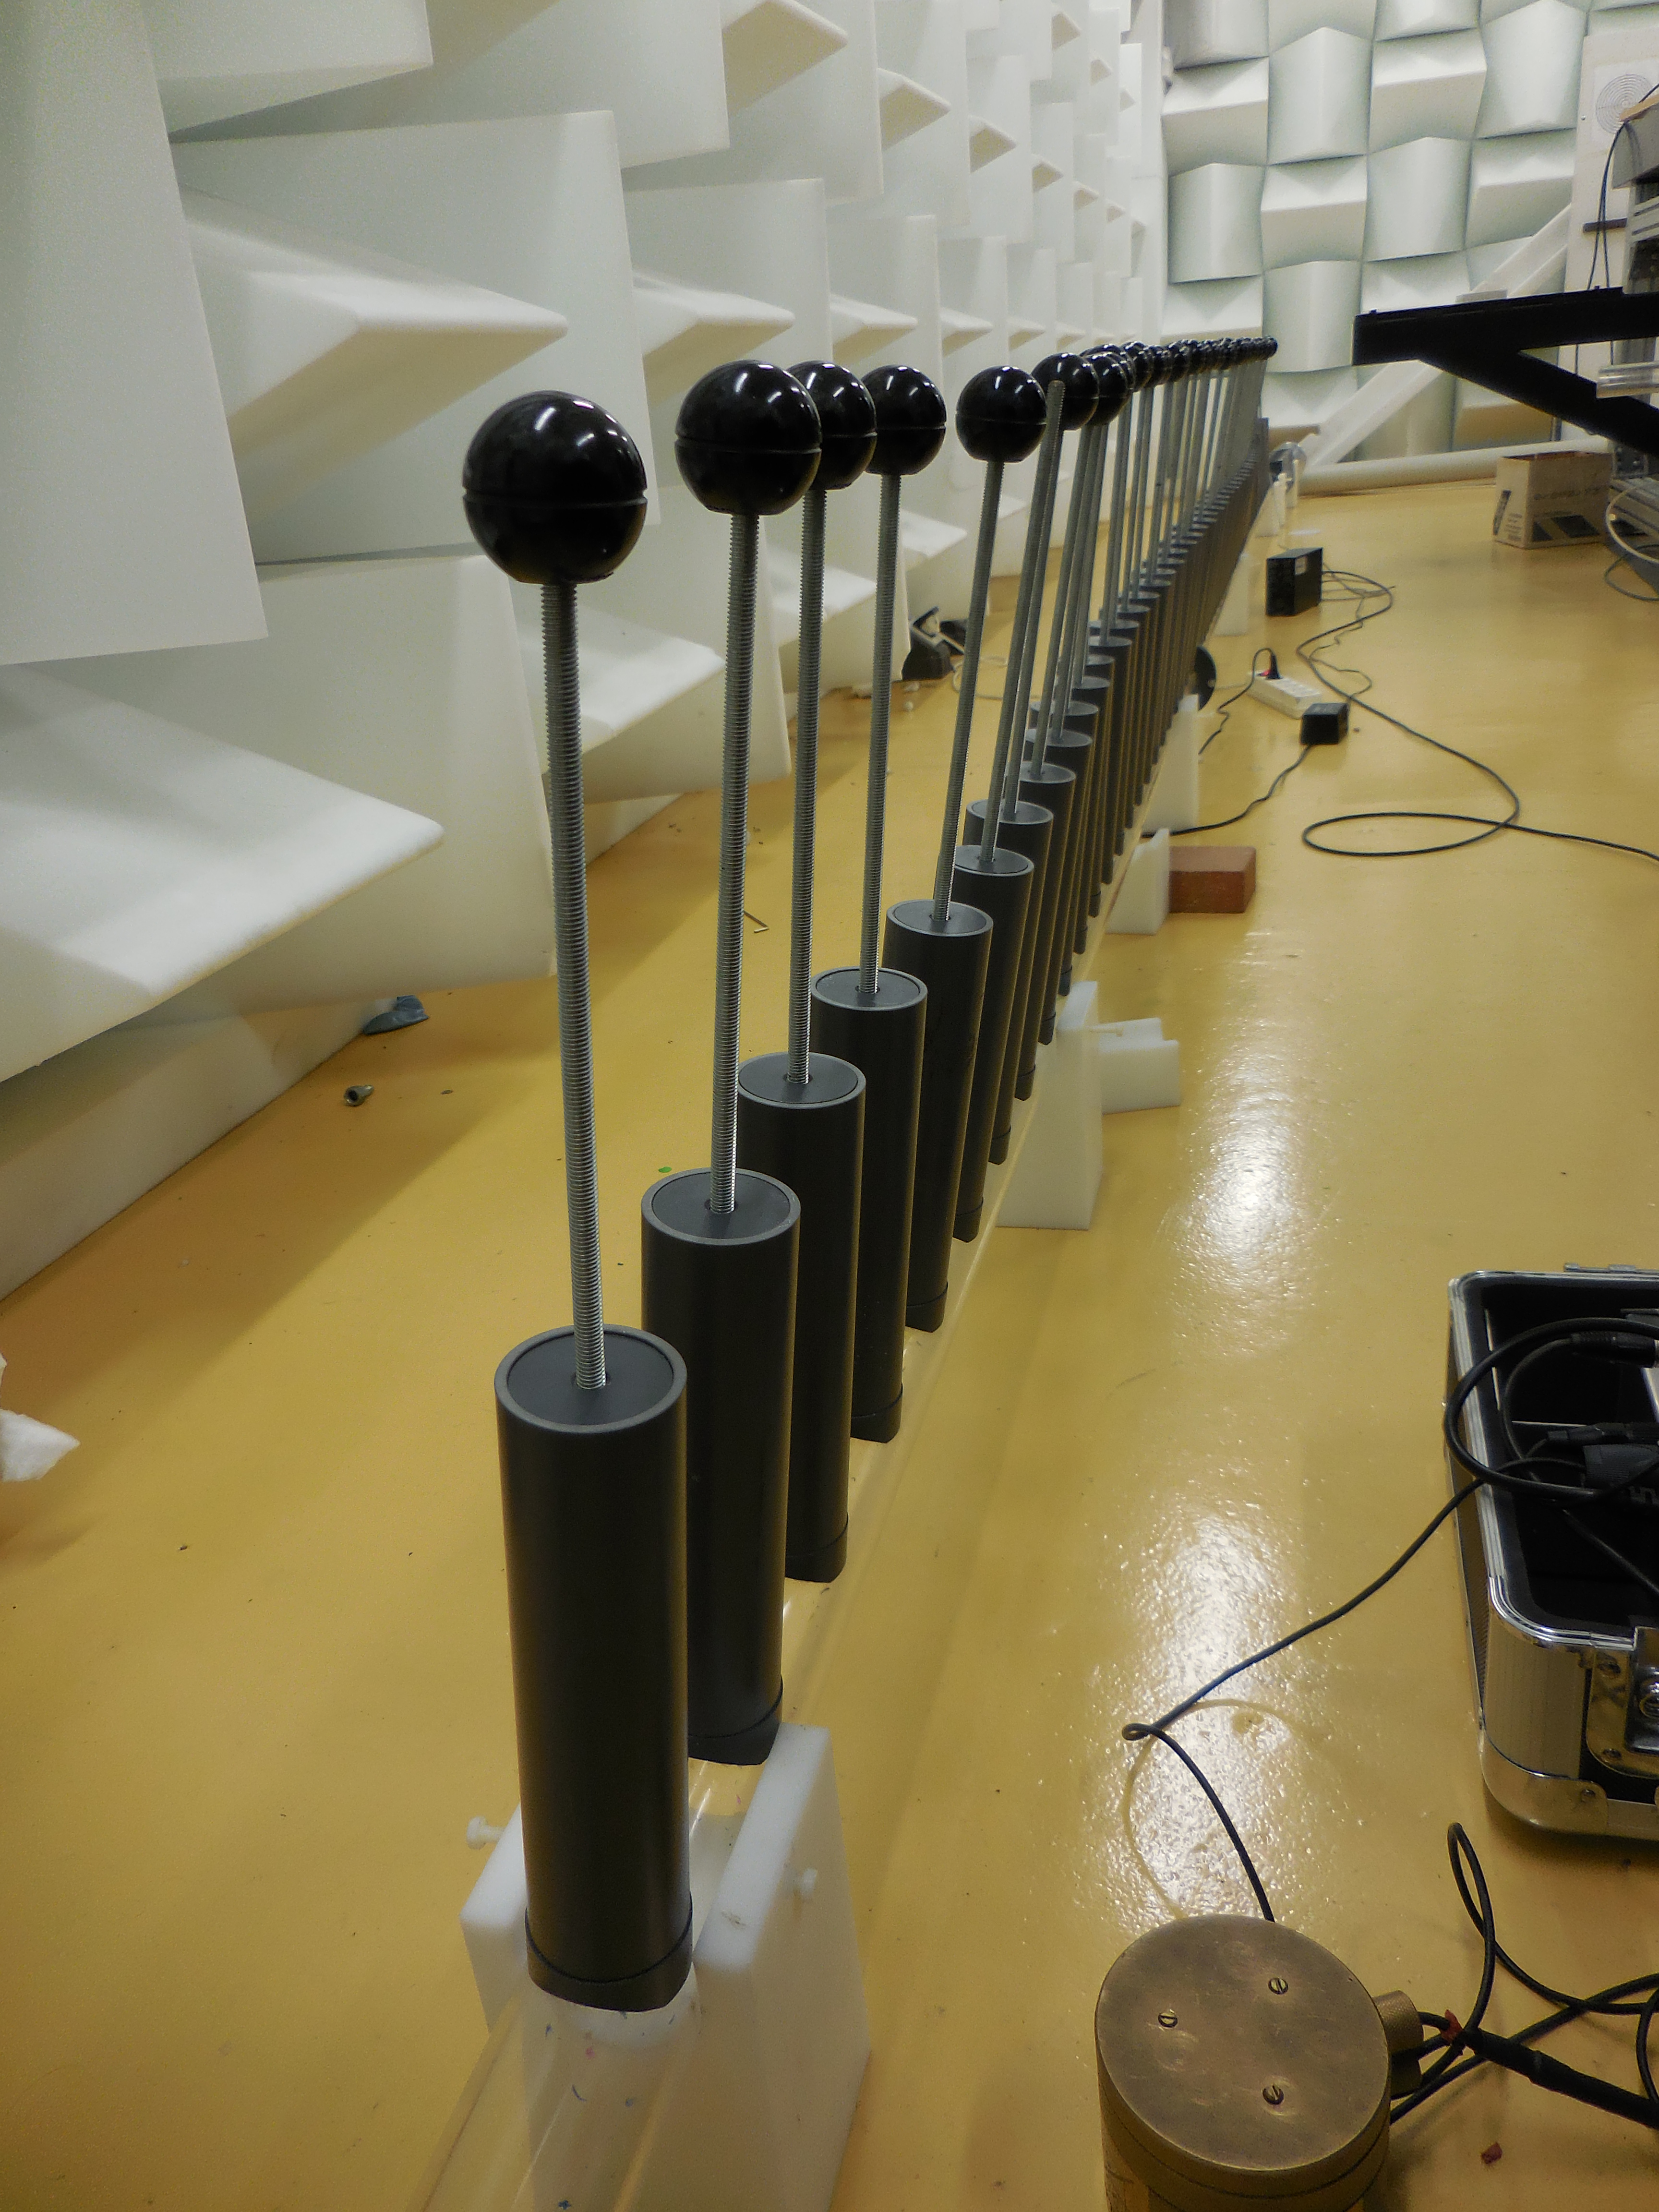
\includegraphics[scale=0.03]{images_chp3/DSCN0123.JPG}
	\caption{Photo du banc de mesure utilisé.\label{photo_manip}}
\end{figure}

Les mesures de pression dans le guide sont faites par déplacement manuel d'un microphone (GRAS 26AC) directement placé à l'intérieur du réseau.

\bigskip

A l'autre extrémité du réseau se trouve une sortie anéchoïque préalablement réglée afin que le coefficient de réflexion au bout du réseau soit le plus faible possible. Le coefficient de réflexion du guide sans les résonateurs est en dessous de 8\% pour la bande de fréquence d'intérêt (cf annexe \ref{term_anecho}).


\section{Mesure du coefficient de réflexion et de transmission du réseau}
On s'intéresse tout d'abord à la mesure du coefficient de réflexion et de transmission dans le réseau. Le but est de chercher la fréquence précise à laquelle le mode de défaut a lieu afin de pouvoir par la suite l'observer expérimentalement. Pour cela, on ne prend que 5 résonateurs (avec un défaut sur le troisième) afin que le mode localisé puisse s'étaler sur les bords du réseau et qu'il soit ainsi visible sur les coefficients de réflexion et de transmission. Les résonateurs ont une longueur de cavité de $16~cm$ et le défaut de $7.5~cm$, et sont espacés de $10~cm$. Les courbes figure~\ref{ref_trans1} et~\ref{ref_reflexion1} correspondent aux coefficients de réflexion et de transmission pour cette configuration, en comparaison avec le cas sans défaut.

\begin{figure}[!h]
	\centering
	\subfigure[Sans défaut]{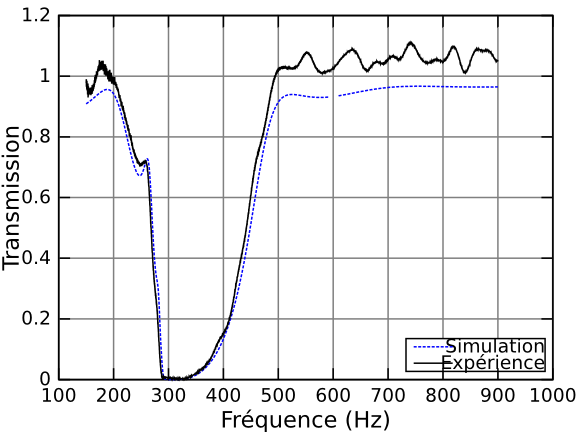
\includegraphics[scale=0.4]{images_chp3/T_5HR165_nodefect.png}}
	\subfigure[Avec un défaut résonant à 485 Hz]{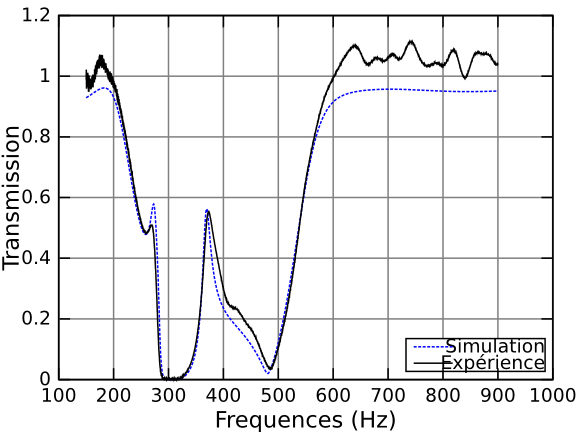
\includegraphics[scale=0.4]{images_chp3/T_5HR165_8cm_pos3.png}}
	\caption{\label{ref_trans1} Coefficients de transmission du réseau dans un cas sans défaut et avec défaut. Les courbes de simulations (tiretée) et de l’expérience (continue) sont superposées.}
\end{figure}

\begin{figure}[!h]
	\centering
	\subfigure[Sans défaut]{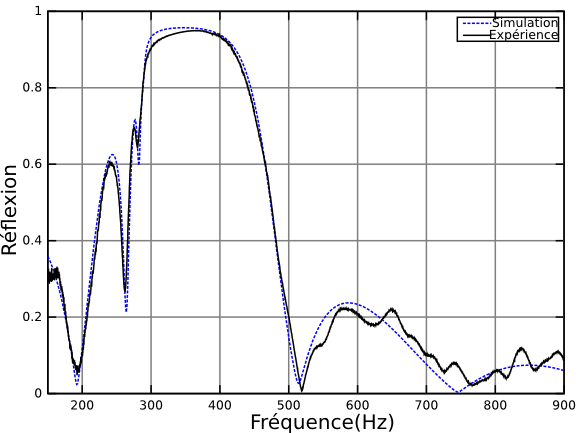
\includegraphics[scale=0.4]{images_chp3/R_5HR165_nodefect.png}}
	\subfigure[Avec un défaut résonant à 485 Hz]{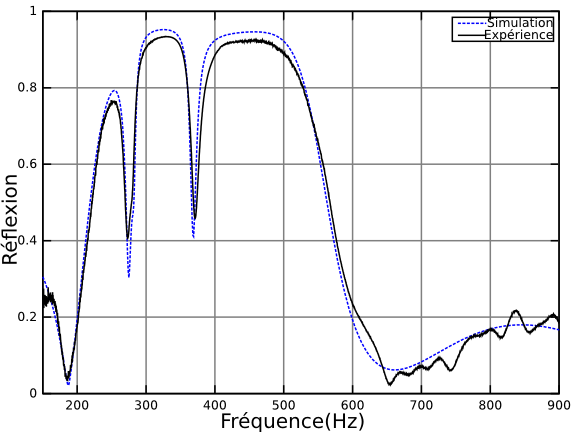
\includegraphics[scale=0.4]{images_chp3/R_5HR165_8cm_pos3.png}}
\caption{\label{ref_reflexion1} Coefficients de réflexion du réseau dans un cas sans défaut et avec défaut. Les courbes de simulations (tiretée) et de l’expérience (continue) sont superposées.}
\end{figure}

Dans l'ensemble, simulations et mesures sont en accord. Certaines variations sont moins marquées sur les courbes expérimentales en raison des fuites aux jonctions du guide et des résonateurs non prises en comptes dans la simulation.\\
Aux fréquences pour lesquelles la transmission est théoriquement proche de 1, il y a de fortes variations observées expérimentalement, allant jusqu'à dépasser 1. Cet écart entre théorie et expérience s'explique par la contribution des faibles réflexions provenant de la terminaison anéchoïque qui n'est pas parfaite.\\~\\


On constate qu'un pic de transmission est visible autour de 370 Hz, dans la bande interdite, tant théoriquement qu'expérimentalement : le défaut amplifie et permet à l'onde de traverser le réseau pour une fréquence donnée, alors que dans le cas sans défaut, aucune transmission n'est possible. Ce comportement laisse supposer qu'un mode localisé est présent au niveau du défaut : si on augmente le nombre de résonateurs, l'atténuation est plus forte et le pic disparaît. Le mode est alors complètement localisé. 

Selon la géométrie du réseau et la fréquence de résonance du défaut, l'effet du mode localisé peut apparaître plus ou moins clairement sur le coefficient de réflexion. Dans le cas des figures~\ref{ref_trans1},~\ref{ref_reflexion1}, le réseau est suffisamment court pour que l'effet du défaut soit aussi bien visible en transmission qu'en réflexion.

La figure~\ref{multiR} montre que l'effet du mode localisé est plus visible quand la fréquence de résonance du défaut se trouve sur le bord d'une bande interdite (ici, à $485~Hz$, pour $L_c=75~mm$). Cette configuration permet que le signal d'excitation ne soit pas trop atténué pendant sa propagation jusqu'au défaut. Il y a alors suffisamment d'énergie pour faire résonner le défaut et que cela soit visible sur le coefficient de transmission.

\begin{figure}[!h]
	\centering
	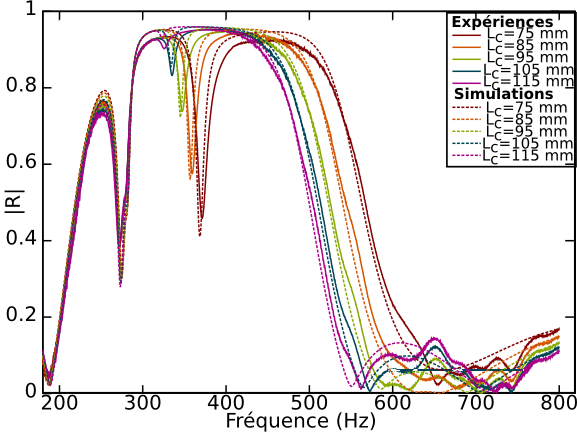
\includegraphics[scale=0.5]{./images_chp3/multiR.png}
	\caption{\label{multiR}Coefficient de réflexion à l'entrée d'un réseau de 5 résonateurs, pour différentes longueurs de cavité du défaut situé en 3\textsuperscript{ème} position.}
\end{figure}



\section{Mesure d'un mode localisé par insertion de capteur dans le réseau}



Le nombre de résonateurs de part et d'autre du défaut est augmenté de manière à créer un mode complètement localisé. Afin de pouvoir quand même exciter le défaut à la fréquence du mode recherché, et ce malgré la longueur du réseau, une source est placée dans un des orifices au voisinage du défaut. Pour des raisons techniques, les résonateurs sont alors espacés de $20~cm$. De plus, pour éviter le bruit en basses fréquences dû à la réponse des transducteurs utilisés, la longueur de cavité des résonateurs est diminuée à $9.5~cm$, permettant ainsi de monter la première bande interdite en fréquence. Enfin, la cavité du défaut est fixée à $8~cm$. Dans ces conditions, les cellules étant plus grandes, l'atténuation dans le guide est plus forte et la fréquence du mode de défaut est moins visible sur les coefficients de transmission et de réflexion. Cependant, avec l'aide d'une simulation, il possible de détecter sur la figure~\ref{ref_loc} une modification de la réflexion quand il y a un défaut. Un pic correspondant au mode de défaut apparaît à $370~Hz$.



 Le signal d'excitation est donc un sinus à $370~Hz$ et un microphone est inséré dans le réseau afin de mesurer la pression en tout point. Le microphone n'est pas intrusif car sa taille (quart de pouce, soit 0.6 cm) est petite devant celle de la longueur d'onde. L'amplitude de la pression mesurée dans le tube est représentée figure~\ref{p_tube} pour une configuration avec et sans défaut. 


\begin{figure}[!h]
	\begin{minipage}[l]{1 \textwidth}
		\subfigure[Avec défaut en 3\textsuperscript{ème} position]{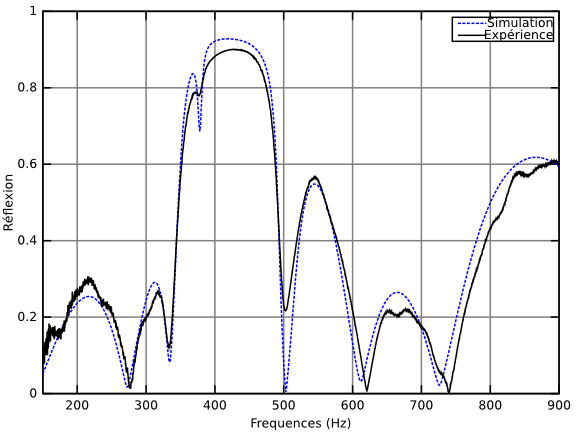
\includegraphics[scale=0.4]{./images_chp3/R_5HR10cm_Lcell20_85mm_pos3.png}}
		\centering
		\subfigure[Sans défaut]{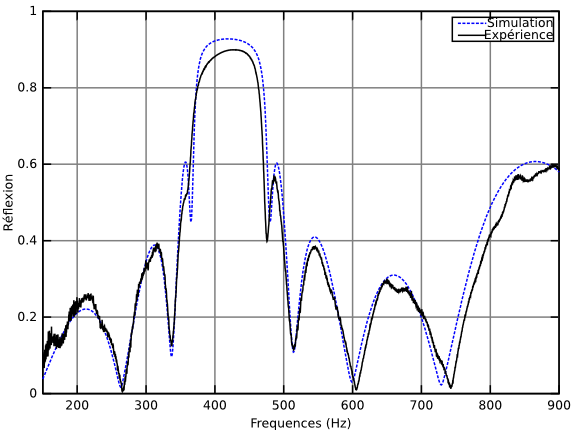
\includegraphics[scale=0.4]{./images_chp3/R_5HR10cm_Lcell20_nodefect.png}}
		\caption{Coefficient de réflexion à l'entrée d'un réseau de 5 cellules.\label{ref_loc}}
	\end{minipage}
	\hspace{0.5cm}
	\begin{minipage}[r]{1 \textwidth}
		\centering
		\subfigure[]{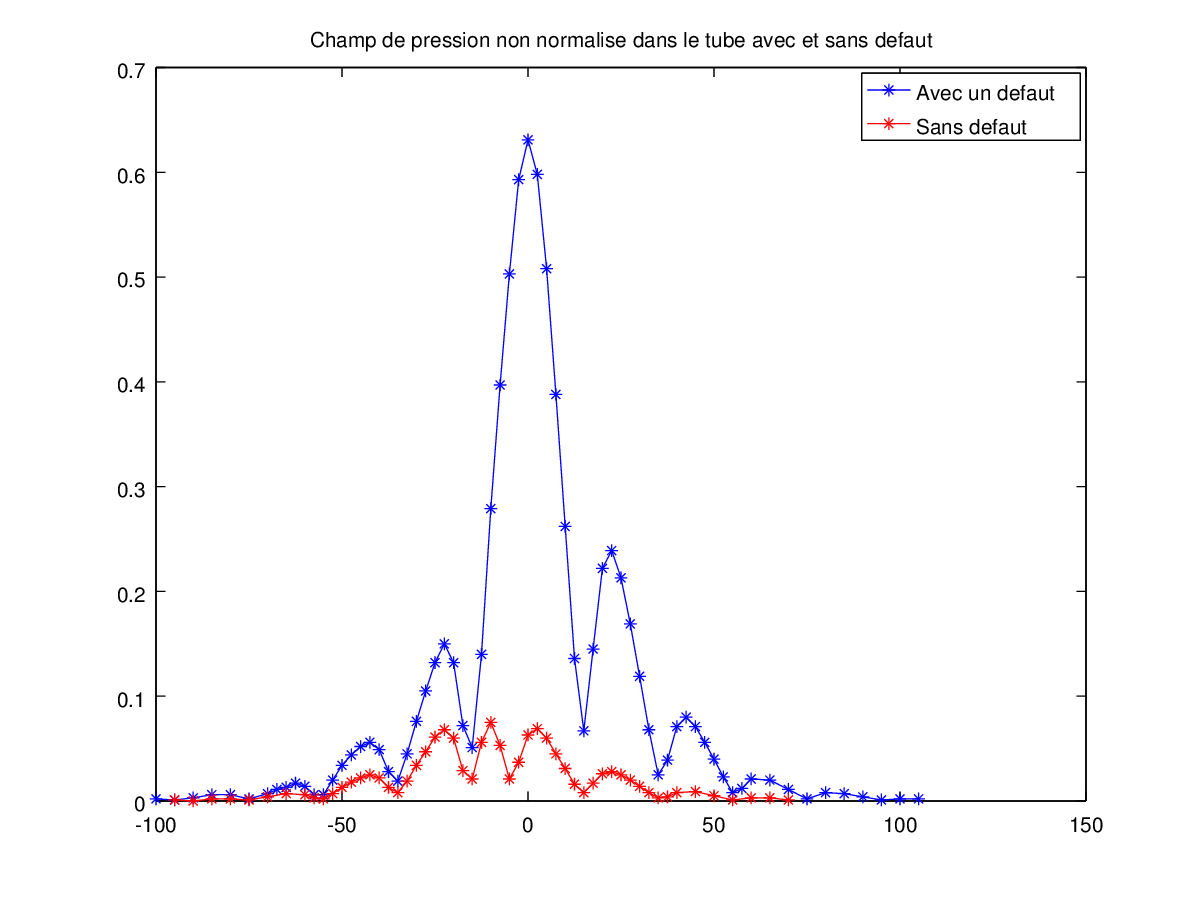
\includegraphics[scale=0.2]{./images_chp3/non_norm_lin.png}}
		\caption{Amplitude du microphone mesurée dans le guide avec et sans défaut.\label{p_tube}}
	\end{minipage}
\end{figure}

Les niveaux de pression mesurés sont près de 10 fois plus élevés dans le cas où un défaut est présent. De plus, la décroissance à mesure que l'on s'éloigne du défaut est très importante : on est donc bien en présence d'un mode localisé. Il est a noter que dans cette configuration, le niveau maximum dans le réseau ne se situe pas au niveau de la source mais au niveau du défaut (ce qui n'est pas le cas quand il n'y a pas de défaut).\\~\\


Pour des questions matérielles, il n'a pas été possible de placer la source au même endroit que le défaut dans le réseau. La symétrie du système n'est donc pas conservée. C'est pourquoi les 2 courbes de la figure \ref{p_tube} ne sont pas centrées sur le même point.

\section{Changement de géométrie du défaut}
Afin de pouvoir comparer la différence de décroissance entre les 2 courbes, on change la géométrie de la cellule singulière : celle-ci est maintenant constituée de 2 résonateurs afin de pouvoir placer la source au centre. Les cellules sont alors constituées de 2 résonateurs (voir schéma figure \ref{fig_exp}). La source se trouve au point $x=0$, les résonateurs ont une longueur de cavité de $16~cm$ et ceux du défaut une longueur de $8~cm$.


Le couplage des deux défauts engendre en réalité deux fréquences de résonance. En prenant des longueurs de cavité plus grandes (16 cm au lieu de 8), l'une d'elle tombe dans une bande interdite, générant ainsi un mode localisé.

\begin{figure}[!h]
\centering
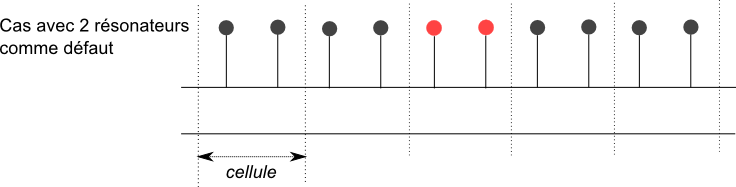
\includegraphics[scale=0.5]{./images_chp3/chgmt_defaut2.png}
\caption{\label{fig_exp} Schéma décrivant le changement du défaut afin de rendre le réseau symétrique.}
\end{figure}



Après avoir effectué ce changement de géométrie, les courbes de pression obtenues sont celles de la figure \ref{p_tube2}.
Les mesures sont comparées avec une courbe de décroissance théorique calculée à partir de l'équation de dispersion~\ref{eq_dispersion} en isolant la constante de propagation $k$. La décroissance est alors donnée par $e^{-\Im{k}x}$ où $x$ est la distance parcourue par l'onde.

\begin{figure}[!h]
\centering
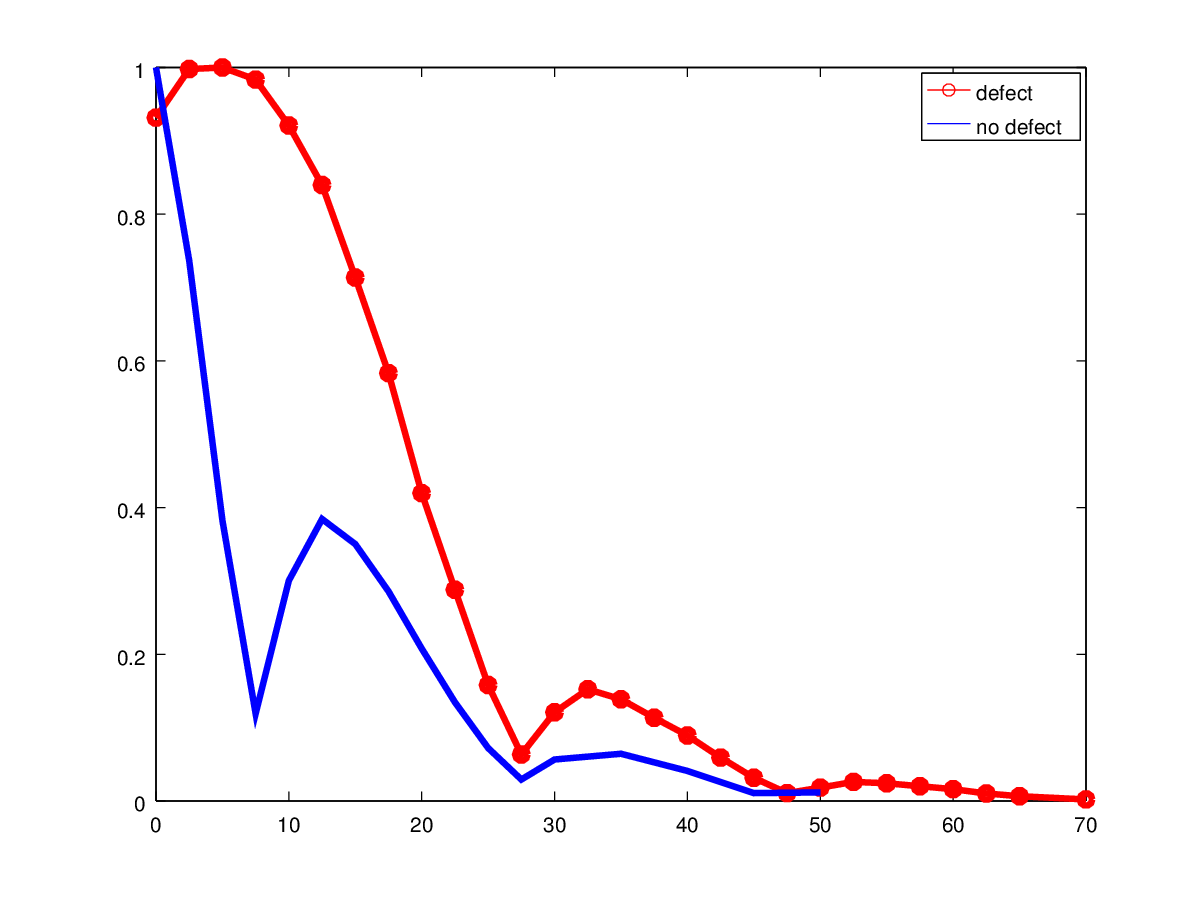
\includegraphics[width=0.5 \textwidth]{./images_chp3/comparaison_decroissance_lin.png}\hfill
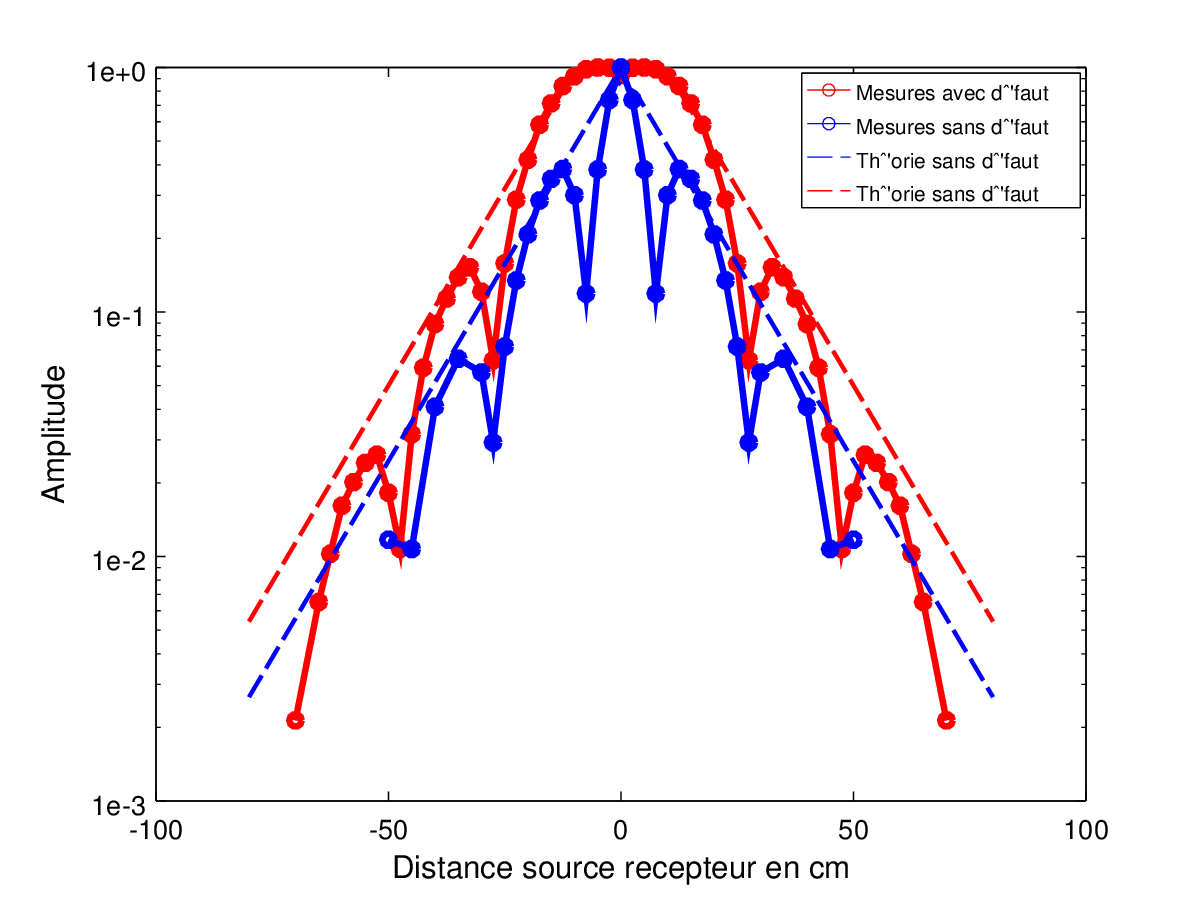
\includegraphics[width=0.5 \textwidth]{./images_chp3/comparaison_decroissance_log_theo.png}
\caption{\label{p_tube2} Amplitude du microphone mesurée dans le réseau avec un défaut à 2 résonateurs. À gauche en échelle linéaire, à droite en échelle logarithmique, la courbe de comparaison des décroissances est normalisée.}
\end{figure}

Tout d'abord il est visible sur la première courbe figure~\ref{p_tube2} que l'amplitude du mode localisé est nettement plus élevée que dans un cas sans défaut. Le résultat de la partie précédente est donc bien retrouvé ici. \\

Dans le cas sans défaut, la décroissance mesurée est légèrement plus importante que celle simulée, en raison des pertes dues aux fuites.
Dans le cas avec défaut, la pression ne décroît pas dans la première cellule (sur les 10 premiers centimètres, correspondant à la distance source-défaut) car le défaut résonne. Il y a ensuite une décroissance équivalente à celle d'un réseau sans défaut.
Une onde de forte amplitude est donc bien localisée au niveau de la singularité. Mais le défaut ne semble pas agir sur le reste du réseau.






\chapter{Conclusion}

Ce projet a permis l'étude d'un réseau périodique de résonateurs de Helmholtz en prenant en compte les pertes visco-thermiques. 

Dans un premier temps, un réseau périodique infini a été étudié afin de se familiariser avec le formalisme matriciel (onde de Bloch): celui-ci est très apte à décrire ce genre de système. Les simulations faites sur la base de ce modèle théorique ont été en parfait accord avec des mesures effectuées sur le banc d'expérience du LAUM\footnote{\samepage Laboratoire d'Acoustique de l'Université du Maine}. Une étude succincte d'un faible désordre dans le réseau a également été abordée : un désordre sur la position des résonateur affecte les bandes de Bragg, tandis qu'un désordre sur la longueur des cavités modifie les bandes interdites liées à l'impédance des résonateurs.

 
Dans un second temps, un défaut a été ajouté dans le réseau afin de générer un mode localisé. Là encore, les simulations sont en accord avec les expériences. Bien que le phénomène soit difficile à observer du fait de la localisation de la pression dans le tube à cause des bandes interdites, les mesures sur un réseau avec un faible nombre de résonateurs ont permis de mettre en évidence l’existence d'un mode de défaut sur les coefficients de transmission et réflexion et de connaître la fréquence exacte d’excitation du mode. Il a alors été possible de mesurer la pression dans le tube en excitant près du défaut à cette fréquence. La différence d'ordre de grandeur des pressions entre un réseau avec et sans défaut s'est montrée flagrante et a corroboré les expériences précédentes, montrant qu'il s'agissait bien d'un mode de défaut.

Ces travaux peuvent avoir pour suite l'ajout de phénomènes non-linéaires afin de créer des filtres intéressant à appliquer dans la création de méta-matériaux. Le résonateur de Helmholtz n'étant pas linéaire pour de grandes amplitudes, sa fréquence de résonance s'abaisse quand l'amplitude augmente (pour de grandes amplitudes). Plusieurs applications peuvent donc découler de ce phénomène.

Par exemple, dans le cas d'un résonateur dont la fréquence est dans une bande interdite en amplitude faible, cette résonance pourra ne plus être dans une bande interdite pour une amplitude plus forte : un filtrage en amplitude est alors possible (filtrage dynamique).


De plus, une génération d'harmoniques supérieurs par ce même résonateur est possible en forte amplitude. Ainsi, si une source excite ce défaut, engendrant des harmoniques supérieurs qui ne sont pas dans une bande interdite, la propagation de ces harmoniques est possible. Mais si ce résonateur est placé loin de la source, l'amplitude d'excitation au niveau du défaut sera très faible, et les harmoniques ne seront pas générés. Il est donc possible de créer des système asymétrique sur ce principe.








\chapter*{Annexes}

\section*{Terminaison anéchoïque}
\label{term_anecho}
La terminaison anéchoïque est constituée de fin tissu métallique résistif auquel vient s'ajouter une cavité de section variable qui crée une discontinuité de section. Afin de fixer cette dernière on procède au calcul du coefficient de réflexion du réseau sans aucun résonateur (juste le tube). Le but est de voir quel est l'impact de l'onde réfléchie par la sortie anéchoïque sur l'entrée du réseau. Après réglage, la courbe de réflexion figure~\ref{fig_term_anecho} est finalement obtenue.

\begin{figure}[!h]
\centering
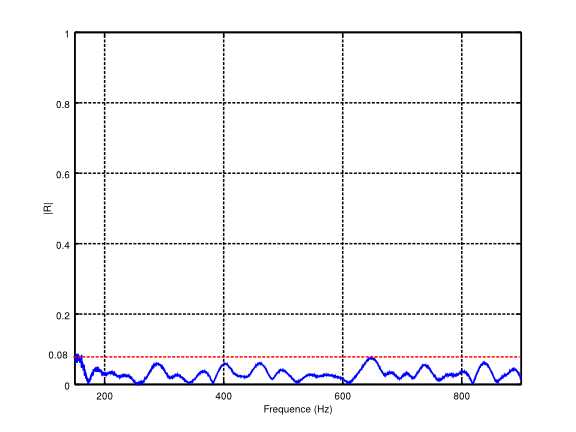
\includegraphics[scale=0.4]{./images_annexe/anecho.png}
\caption{\label{fig_term_anecho} Coefficient de réflexion pour le réseau sans résonateur avec une terminaison anéchoïque adaptée.}
\end{figure}

On constate que le coefficient de réflexion ne dépasse jamais 0.08 ce qui semble tout à fait acceptable afin de considérer la sortie comme anéchoïque dans le reste du projet.

\section*{Paramètres du réseau étudié}
\label{annexe_corr}
La liste des dimensions du réseau utilisé lors des expériences et des simulations est la suivante:
\begin{itemize}
\item Le guide a un rayon de $R_t = 2.5~cm$ et une épaisseur de $ep = 0.5~cm$.
\item Les résonateurs sont composés de 2 tubes: le col de $R_n = 1~cm$ de rayon et $L_n = 2~cm$ de longueur, la cavité de $R_c = 2.15~cm$ de rayon et de longueur variable $L_c$. C'est cette dernière longueur qui permet de faire varier la fréquence de résonance du résonateur. 
\end{itemize}

\bigskip
Les corrections apportées aux cols des résonateurs sont les suivantes:
\begin{eqnarray*}
l_1 & = &  0.82 \left[ 1 - 1.35 \frac{R_n}{R_c} + 0.31 \left(\frac{R_n}{R_c} \right)^3  \right] R_n \\
l_2 & = &  0.82 \left[ 1 - 0.235 \frac{R_n}{R_t} - 1.32 \left( \frac{R_n}{R_t} \right)^2 +1.54 \left( \frac{R_n}{R_t}\right)^3 - 0.86 \left( \frac{R_n}{R_t}\right)^4  \right] R_n \\
L_{corr} & = &  l_1 + l_2
\end{eqnarray*}
Celles-ci sont dues aux discontinuités de section à l'entrée et la sortie du col. Ces discontinuités entraînent une augmentation de la longueur effective de part et d'autre du col.
\textbf{Notations}

résonateurs : 
$L_{n}$ : longueur du col\\
$R_{n}$ : rayon du col\\
$L_{c}$ : longueur de la cavité\\
$R_{c}$ : rayon de la cavité\\
$S_{n}$ : section du col\\
$S_{c}$ : section de la cavité\\
$Z_{c}$ : impédances carac du col. De même pour n\\

impédance quelconque au point $x_{0}$ : $Z(x_{0})$\\

impédance du résonateur : $Z_{r}$\\

Longueur de la cavité singulière : $L_{c_{s}}$\\ 





\bibliographystyle{plain}
\bibliography{biblio}
\end{document}